\documentclass[aspectratio=169]{beamer}
\usepackage[utf8]{inputenc}
\usepackage[T5]{fontenc}
\usepackage[vietnamese]{babel}
\usepackage{graphicx}
\usepackage{hyperref}
\usepackage{lmodern}

% Theme
\usetheme{Madrid}
\usecolortheme{whale}

% Metadata
\title[Đạo đức trong AI Nông nghiệp]{Đạo đức trong việc sử dụng AI và Dữ liệu lớn trong Nông nghiệp}
\subtitle{Nghiên cứu trường hợp của một Tập đoàn Nông nghiệp Đa quốc gia}
\author{Giảng viên}
\institute{Đại học Đông Á}
\date{\today}

\begin{document}

\begin{frame}
    \titlepage
\end{frame}

\begin{frame}{Nội dung chính}
    \tableofcontents
\end{frame}

\section{Giới thiệu chung}
\begin{frame}{Giới thiệu chung}
    \begin{itemize}
        \item Ngành nông nghiệp chiếm gần 26,5\% dân số thế giới và cần tăng 70\% sản lượng vào năm 2050.
        \item Hệ thống Thông tin Thông minh (SIS), tích hợp Dữ liệu lớn (Big Data) và AI, là giải pháp hứa hẹn để giải quyết bài toán an ninh lương thực.
        \item \textbf{Lợi ích của SIS}: Tự động hóa, giảm chi phí, dự báo nhanh, cải thiện ra quyết định.
        \item \textbf{Các lo ngại tiềm ẩn}:
        \begin{itemize}
            \item Tính chính xác của dữ liệu và khuyến nghị.
            \item Xung đột quyền sở hữu dữ liệu và tài sản trí tuệ.
            \item Sự phân chia kỹ thuật số (người giàu - người nghèo).
            \item Quyền riêng tư và an ninh.
        \end{itemize}
    \end{itemize}
\end{frame}

\section{Sử dụng SIS và Thu thập dữ liệu}
\begin{frame}{Việc sử dụng SIS trong Nông nghiệp}
    \begin{figure}[h]
        \centering
        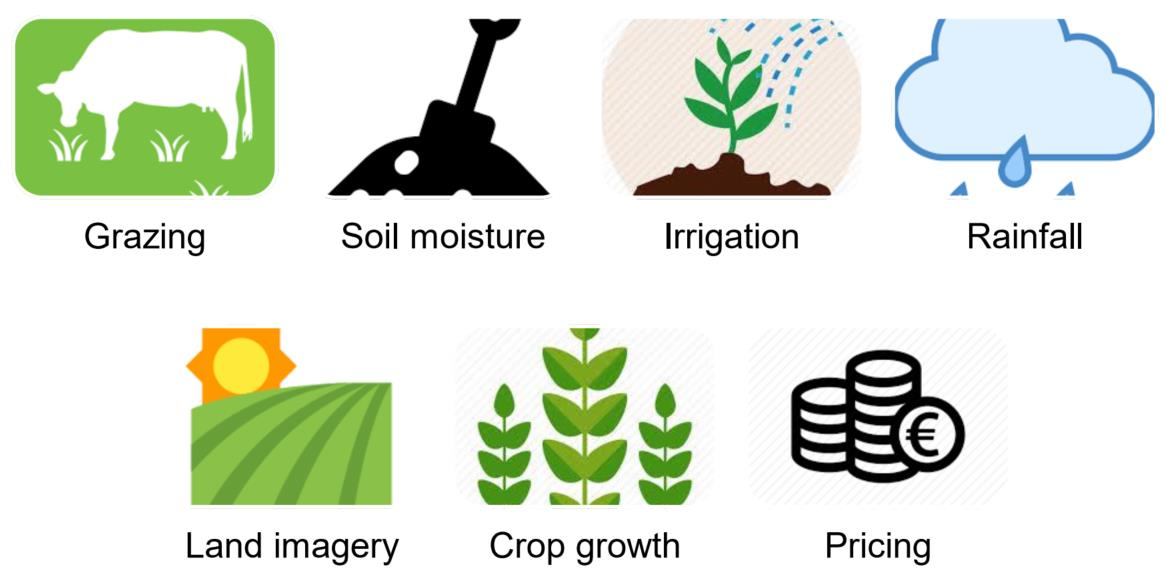
\includegraphics[height=0.6\textheight]{images/ethics_p4_1.jpeg}
        \caption{Hình 1: Các loại Dữ liệu Nông nghiệp được Thu thập (Chăn thả, Độ ẩm, Khí hậu...)}
    \end{figure}
\end{frame}

\begin{frame}{Các lĩnh vực hứa hẹn được cải thiện}
    \begin{figure}[h]
        \centering
        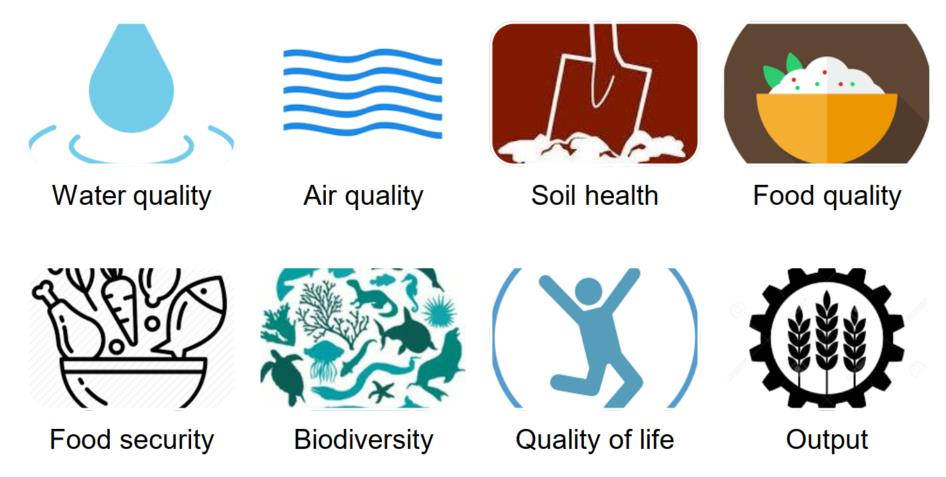
\includegraphics[height=0.6\textheight]{images/ethics_p5_1.jpeg}
        \caption{Hình 2: Các lĩnh vực nông nghiệp được cải thiện nhờ Dữ liệu lớn}
    \end{figure}
\end{frame}

\section{Các vấn đề Đạo đức trong Lý thuyết}
\begin{frame}{Các vấn đề Đạo đức khi sử dụng SIS}
    \begin{figure}[h]
        \centering
        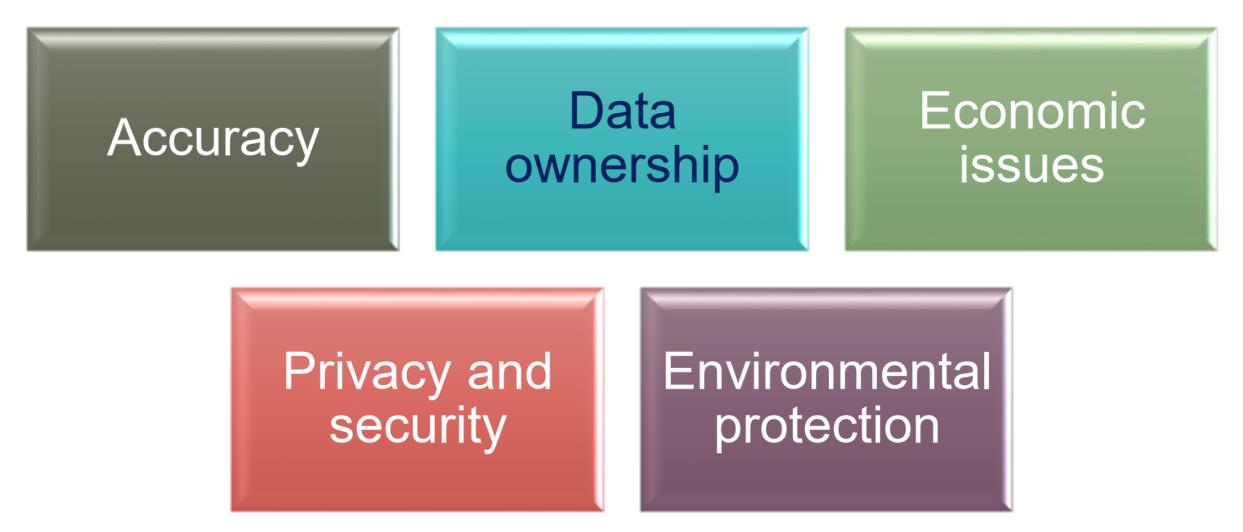
\includegraphics[height=0.6\textheight]{images/ethics_p7_1.jpeg}
        \caption{Hình 3: 5 vấn đề đạo đức chính trong Tài liệu lý thuyết}
    \end{figure}
\end{frame}

\begin{frame}{1. Tính chính xác của Dữ liệu và Khuyến nghị}
    \begin{itemize}
        \item Các thuật toán AI đôi khi không cân bằng được tính kịp thời và tính chính xác, dẫn đến kết luận sai lệch.
        \item Môi trường thời tiết (nhiệt độ khắc nghiệt, độ ẩm) có thể làm sai lệch kết quả đọc của cảm biến.
        \item Nếu thuật toán không tính đến đặc thù địa phương, khuyến nghị đưa ra có thể gây mất mùa, vật nuôi mắc bệnh và thiệt hại kinh tế.
    \end{itemize}
\end{frame}

\begin{frame}{2. Quyền sở hữu Dữ liệu và Sở hữu Trí tuệ}
    \begin{itemize}
        \item \textbf{Nỗi lo của nông dân}: Dữ liệu bị bán cho nhà giao dịch hàng hóa, cơ quan quản lý hoặc bị sử dụng để ép giá.
        \item Các nhà cung cấp công nghệ (ATP) thường cấp giấy phép "miễn phí bản quyền" để họ có thể sử dụng dữ liệu của nông dân.
        \item Nông dân nhỏ thiếu kiến thức pháp lý và khả năng thương lượng hợp đồng.
        \item Nông dân không được sửa chữa máy móc (ví dụ: máy kéo John Deere) vì vi phạm sở hữu trí tuệ phần cứng/phần mềm.
    \end{itemize}
\end{frame}

\begin{frame}{3. Các vấn đề Kinh tế và Phân chia Kỹ thuật số}
    \begin{itemize}
        \item Các trang trại nhỏ chiếm số lượng lớn nhưng ít tiếp cận công nghệ do chi phí cao.
        \item Gây ra sự \textbf{phân chia kỹ thuật số}: Bất bình đẳng gia tăng giữa các trang trại công nghiệp lớn và nông hộ nghèo.
        \item Ở các nước đang phát triển (LMIC): Khó triển khai SIS do hạ tầng yếu kém, thiếu kỹ năng, thiếu khung pháp lý bảo vệ dữ liệu.
    \end{itemize}
\end{frame}

\begin{frame}{4. Quyền riêng tư \& 5. Bảo vệ môi trường}
    \begin{itemize}
        \item \textbf{Quyền riêng tư \& An ninh}:
        \begin{itemize}
            \item Thu thập dữ liệu nhạy cảm (thu nhập, địa điểm, năng suất).
            \item Drone xâm phạm quyền riêng tư của bên thứ ba.
            \item Dễ bị lạm dụng bởi đối thủ cạnh tranh hoặc tin tặc.
        \end{itemize}
        \item \textbf{Phúc lợi Động vật \& Bảo vệ Môi trường}:
        \begin{itemize}
            \item Thiết bị điện tử (vòng cổ, cảm biến) có thể gây thương tích hoặc căng thẳng cho vật nuôi.
            \item Drone/Robot có thể xả thải chất độc hại.
            \item Khuyến nghị tăng sản lượng có thể gây ô nhiễm nguồn nước hoặc xâm lấn hệ sinh thái xung quanh.
        \end{itemize}
    \end{itemize}
\end{frame}

\section{Nghiên cứu tình huống}
\begin{frame}{Nghiên cứu tình huống: Công ty Đa quốc gia Lớn}
    Phỏng vấn 3 nhân sự cấp cao tại một tập đoàn đa quốc gia đang triển khai dự án SIS.
    \begin{figure}[h]
        \centering
        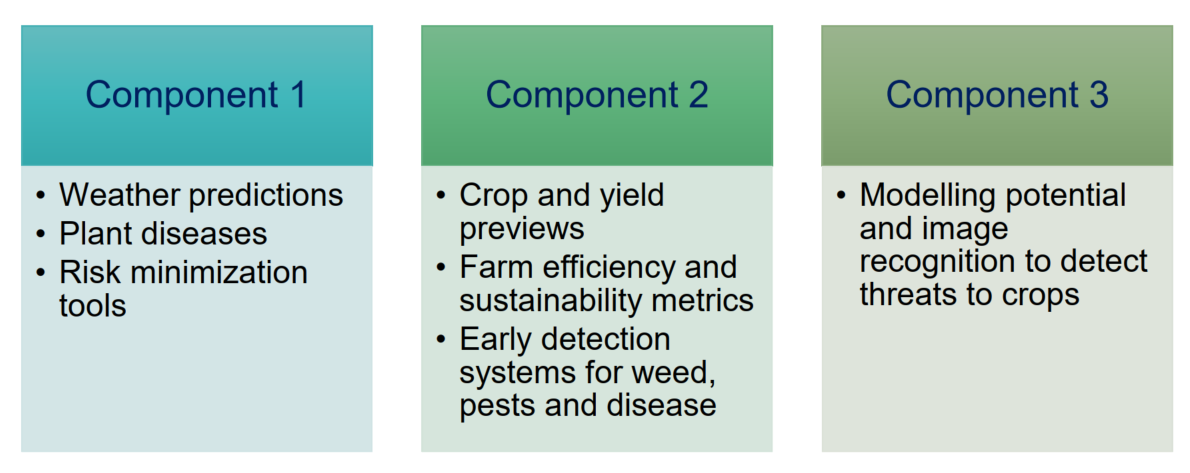
\includegraphics[height=0.45\textheight]{images/ethics_p12_1.png}
        \caption{Hình 4: 3 Thành phần SIS của công ty (Dự báo thời tiết, Năng suất, Hỗ trợ tư vấn)}
    \end{figure}
\end{frame}

\begin{frame}{Các vấn đề Đạo đức tại Công ty}
    \begin{figure}[h]
        \centering
        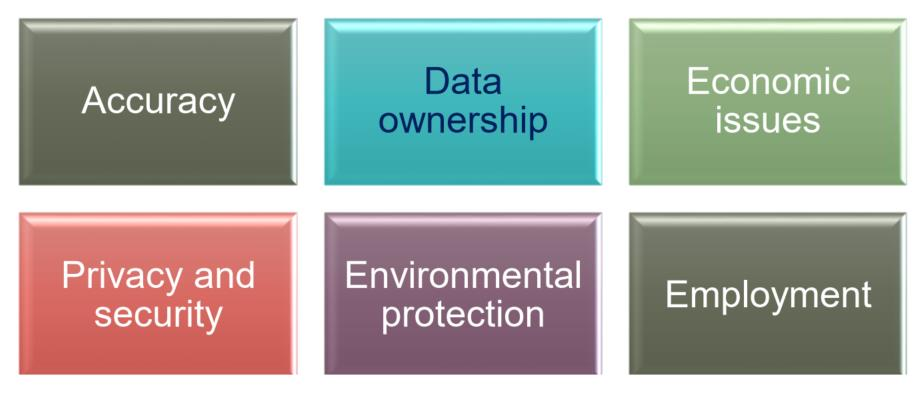
\includegraphics[height=0.5\textheight]{images/ethics_p15_1.jpeg}
        \caption{Hình 5: Các vấn đề đạo đức được xác định trong thực tế tại công ty}
    \end{figure}
\end{frame}

\begin{frame}{So sánh Thực tế và Lý thuyết}
    \begin{itemize}
        \item \textbf{Việc làm}: Thực tế, SIS không thay thế nhà nông học mà đóng vai trò là "công cụ bổ sung". Nông dân vẫn tin tưởng con người hơn phần mềm vô cảm.
        \item \textbf{Quyền sở hữu}: Công ty cam kết người nông dân giữ quyền sở hữu dữ liệu của mình.
        \item \textbf{An ninh dữ liệu}: Mật khẩu và cơ sở dữ liệu được mã hóa cao để chống hacker.
        \item \textbf{Tính chính xác}: Thuật toán nhận diện bệnh cây trồng (ví dụ: lá chuối) chỉ hoạt động tốt nếu có đủ kho dữ liệu huấn luyện rõ nét. Sự can thiệp của con người là bắt buộc khi có ngoại lệ.
    \end{itemize}
\end{frame}

\section{Kết luận}
\begin{frame}{Kết luận \& Ý nghĩa}
    \begin{block}{Kết luận}
        Mặc dù có nhiều lo ngại về đạo đức (tính chính xác, bảo mật, kinh tế), các công ty lớn đang nỗ lực điều chỉnh SIS để tuân thủ tính minh bạch, bảo vệ dữ liệu nông dân và hướng tới phát triển bền vững.
    \end{block}
    
    \vspace{0.3cm}
    \textbf{Ý nghĩa của báo cáo}:
    \begin{itemize}
        \item Đặt ra vấn đề về "trách nhiệm pháp lý": Ai sẽ chịu trách nhiệm khi SIS đưa ra khuyến nghị sai gây mất mùa?
        \item Nhấn mạnh tầm quan trọng của việc "đồng thuận đầy đủ thông tin" giữa công ty công nghệ và người nông dân.
    \end{itemize}
\end{frame}

\begin{frame}
    \centering \Huge \textbf{Xin Cảm Ơn!}
\end{frame}

\end{document}
